%% the main definitions for the report (KOMA-Script based)
\documentclass[11pt,a4paper,titlepage]{scrreprt}
\usepackage[T1]{fontenc}
\usepackage[utf8]{inputenc}
\usepackage[german,english]{babel}
%\usepackage{layouts}
\usepackage{graphicx}

\begin{document}

\selectlanguage{\german}

\title{{\Huge \bf MVC}\\[0.55em]{\LARGE Der Model-View-Controller}}
\author{SE3 Team --- Silvio Kunaschk}

\date{\today}
\maketitle

\begin{abstract}
Das ist der Beleg zur wo-Vorlesung Software-Engineering 3 an der HTW-Dresden im SS09.

...

\end{abstract}

\tableofcontents

\chapter{Allgemeine Betrachtungen}
In der Entwicklung von Software-Systemen haben sich (letztendlich) die Systeme durchgesetzt, 
welche mit Hilfe von graphischen Bedienoberflächen es dem Benutzer erlauben, das System
bzw. eine Anwendung, interaktiv und nutzerfreundlich zu bedienen.\\
Dem Benutzer wird dadurch ein einfacher Zugriff auf das Software-System ermöglicht und
dabei geholfen, eine Anwendung zu verstehen und schneller und komfortabler damit zu arbeiten.

An der Akzeptanz und Verbreitung von Computer-Systemen in nahezu allen Bereichen der Industrie
und Wirtschaft, und in letzter Zeit auch immer mehr im privaten gesellschaftlichen Bereich, und
der (sehr wahrscheinlichen) Annahme, dass die meisten Anwender nur über rudimentäre
Informatikkenntnisse verfügen, aber trotzdem in der Lage sind mit Hilfe der graphischen
Benutzerschnittstelle die verschiedensten Aufgaben mit Software-Systemen einfach und effizient
zu lösen, kann man erkennen, welchen Stellenwert dieser Bestandteil von interaktiven
Software-Systemen besitzt.

Möchte man, dass sich sein Anwendungssystem bzw. Applikation durchsetzt, ist es heutzutage
unabdingbar eine ausgefeilte Benutzerschnittstelle mit zu implementieren, oder aber 
das System so zu entwickeln, dass dies von jeweiligen Fachleuten übernommen werden kann.

Spezifiziert man die Architektur eines interaktiven Software-Systems, muß man den funktionalen
Teil von der Bedienschnittstelle unabhängig halten. So können Änderungen an den Teilen
unabhängig voneinander durchgeführt werden, z.B. um die Benutzerschnittstelle an andere
Bedürfnisse anzupassen, ohne Auswirkungen auf den Funktionalen Teil des Systems.

Für diese grundlegende strukurelle Organisation interaktiver Software-Systeme wendet man
das Architekturmuster Model-View-Controller an.

\chapter{Das Model-View-Controller Muster}
\section{Das MVC Paradigma}
\begin{figure}[h]
\fbox{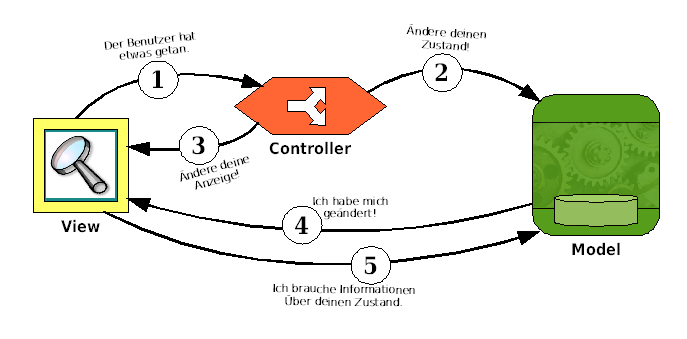
\includegraphics[width=14cm]{mvc-schema.png}}
\caption{Die MVC Komponenten in Aktion}
\end{figure}
Das Model-View-Controller Muster teilt eine interaktive Anwendung in drei Komponenten auf.

Das Model stellt das Anwendungsobjekt dar. Es enthält die gesamte Daten, Zustands-
und Anwendungslogik. Es weiß nichts über Views und Controller, es bietet allerdings eine
Schnittstelle an, über die sein Zustand beeinflußt und abgerufen werden kann. Außerdem
kann es Benachrichtigungen über seine Zustandsänderungen an seine Beobachter senden.

Die View ist die Bildschirmrepräsentation des Anwendungsobjektes. Sie erhält den Zustand
und die Daten (normalerweise) direkt vom Model.

Der Controller bestimmt die Möglichkeiten, mit denen die Benutzungsschnittstelle auf
Benutzereingaben reagieren kann. Er nimmt die Eingaben des Benutzers entgegen und stellt
fest, was diese für das Model bedeuten. Er verarbeitet die Bedieneingaben.

Die View- und die Controllerkomponente beschreiben zusammen die Bedienschnittstelle.
Ein Benachrichtigungsmechanismus sichert die Konsistenz zwischen der Bedienschnittstelle
und dem Model.

Das MVC-Paradigma entkoppelt die Benutzungsschnittstellen der View vom Model. Dies
erhöht die Flexibilität und die Wiederverwendbarkeit.

\section{Das MVC etwas genauer betrachtet}
Schaut man beim Model-View-Controller etwas genauer hin, erkennt man, dass das MVC
ein Satz von Mustern ist, die in einem Entwurf zusammenarbeiten.\\
Es besteht eigentlich aus 3 Entwurfsmustern die hier aber nur kurz erläutert werden
sollen.

\subsection{Observer-Muster}
Das wichtigste Muster beim MVC-Entwurf ist das Observer-Muster. 

Definiere eine 1-zu-n-Abhängigkeit, zwischen Objekten, so dass die Änderung des
Zustands eines Objektes dazu führt, dass alle abhängigen Objekte benachrichtigt
und automatisch aktualisiert werden.

(Bsp. Scema + Klassendiagramm)

... wichtig für das Grundverständnis


\subsection{Strategy-Muster}
Das Strategy-Muster ist - macht - ... zwischen View und Controller! 

Definiere eine Familie von Algorithmen, kapsele jeden einzelnen und mache sie austauschbar.
Das Strategy-Muster ermöglicht es, den Algorithmus unabhängig von ihn nutzenden Klienten
zu variieren.

(Schema - Bild)

Die View delegiert die Verarbeitung der Benutzeraktionen an den Controller. Der Controller
übersetzt die Eingaben des Benutzers in Aktionen auf dem Model.


\subsection{Composite-Muster}
Die View ist ein Kompositum aus GUI-Komponenten (Labels, Buttons, Texteingabefentern, usw. ).
Die oberste Komponente enthält andere Komponenten, die wiederum weitere Komponenten enthalten,
bis man beim Blattknoten angelangt ist.


\section{Nachteile von MVC}


\chapter{Klassenbibliotheken, Toolkit}
\section{XYZ?}
Eine Klassenbibliothek besteht aus einer Menge von verwandten und wiederverwendbaren Klassen,
die entworfen wurden, um nützliche und allgemeine Funktionalität Verfügung zu stellen.
Klassenbibliotheken erwzingen keine bestimmte Anwendungsarchitektur, sie bieten lediglich die
Funktionalität an, mit deren Hilfe eine Anwendung seine Aufgaben erfüllen kann. Bei der
Implementierung braucht man nicht jedes mal das Rad neu zu erfinden.

Damit eine Klassenbibliothek nützlich ist, muß sie in mehreren Anwendungen verwendbar sein.
Daher ist es sehr wichtig, dass sie Annahmen und Abhängigkeiten vermeidet, welche die Flexibilität
und somit die Anwendbarkeit und Effektivität einschränken.

\section{Framwork}
Ein Framework besteht aus einer Menge von zusammenarbeitenden Klassen, die in einem
wiederverwendbaren Entwurf für eine bestimmte Klasse von Software darstellen.\\
Das Framework bestimmt die Architektur der Anwendung.\\
Es definiert:
	- die Struktur im Großen
	- Unterteilung in Klassen und Objekte
	- die jeweiligen zentralen Zuständigkeiten
	- die Zusammenarbeit der Klassen und Objekte sowie den Kontrollfluß

Ein Framework legt diese Entwurfsparameter im voraus fest, so dass der Entwickler
sich auf die spezifischen Details seiner Anwendung konzentrieren kann.\\
Verwendet man ein Framework, schreibt man den Code, der vom Framework gerufen wird.
Dies wird erreicht indem man Operationen mit bestimmten Namen und Aufrufkonventionen
schreiben muß. Dies reduziert die zu treffenden Entwurfsentscheidungen. Diese sind
bereits von anderen getroffen worden.

... das hier in Sätze umformulieren !!!
 - Kreativität
 + "Optimalität", erprobtes, Erfahrung, --> bekannte Verhaltensweisen (für die Benutzer)
 speziell für GUI-Frameworks, Toolkits
 + schnelleres Entwickeln von Anwendungen
 + ähnliche Struktur, einfacher Wiederverwendbar

\chapter{Das Model/View Programming Framework von Qt}
\section{und noch ne Section}
\end{document}
